\section{Exercício 21}

 Faça um programa que calcule a multiplicação de todos os elementos da diagonal
 principal de uma matriz 5x5. Obs.: o algoritmo deve ser genérico para qualquer
 matriz quadrada. Este programa deve chamar uma função para fazer a
 multiplicação

\subsection{Descrição Alto Nível}

A desrição em alto nível foi utilizando a linguagem python é desta forma:

\begin{lstlisting}

def diag(matrix):
    res = 1
    for i in range(len(matrix)):
        el = matrix[i][i]
        res = mult_sum(res, el)
    return res


def mult_sum(a, b):
    res = 0
    while b > 0:
        res += a
        b-=1
    return res

\end{lstlisting}

\subsection{Descrição Baixo nível}
\begin{verbatim}
    
.CODE
	lda	size
	JZ	FIM
	sta	aux
	lda	aux
INIT:
	jz	FIM,R
	lda	m
	add	mov
	sta	value
	jsr	MULT_SUM,R
	lda	mov
	add	#1
	add	size
	sta	mov
	lda	aux
	add	#-1
	sta	aux
	JMP	INIT,r
		MULT_SUM:
			lda	#0
			sta	multAux
			lda	value,I
			sta	val
			LOOP:
				jz	RETURN,R
				add	#-1
				sta	value
				lda	multAux	
				add	res
				sta	multAux
				lda	value
				jmp	LOOP,R
			RETURN:
				lda multAux
				sta res
				rts
FIM:
	hlt
.ENDCODE

.DATA

	res:	db	#1
	size:	db	#5    	
	m:	db	a, b, c, d, e
	a:	db	#1, #6, #7, #8, #9
	b:	db	#10, #2, #11, #12, #13
	c:	db	#14, #8, #3, #16, #17
	d:	db	#18, #19, #20, #4, #21
	e:	db	#22, #23, #24, #25, #5
	aux:	db	#0
	mov:	db	#0
	value:	db	#0
	multAux:db	#0
	val:	db	#0

.ENDDATA

\end{verbatim}

\subsection{Tela Montador}

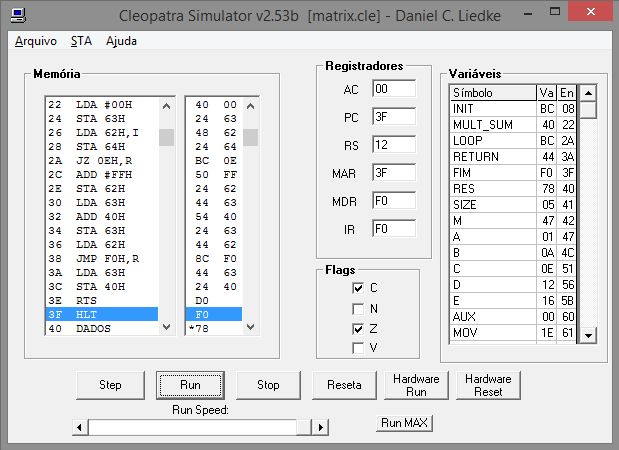
\includegraphics{images/matrix.png}

\subsection{Contagem Operações e estimativa de de tempo de execução}

Considerando \emph{n} como \emph{x} temos a seguinte função:
$$f(x) = 196x + 32$$
O Tempo de excução seria xxx ao considerarmos que o Cleópatra opera a
1GHz.

